%Also, for most of 5.2, you need to make the case that the single result you show
%is representative!!  I think that's easy, but needs to be done.  Essentially,
%you need to make the case that for real isotopes, the same model will be
%invoked with real parameters, so that these normalized (relative?) parameters
%are representative of all cases.

To verify the fundamental behavior of all four \Cyder radionuclide transport models at
each component interface, many transport and containment base cases were
conducted.

The simulations were conducted within the \Cyclus framework and had the
following simulation parameters:

\begin{itemize}
\item{A 1000 year simulation}
\item{A source facility providing one waste stream per time step}
\item{An initial capacity of five 1 kg waste streams (in most cases)}
\item{No more than one waste stream object is stored per waste form}
\item{Corresponding waste package components, one per waste form}
\item{A buffer component (i.e. a bentonite clay)}
\item{A far field component (i.e. the host rock)}
\end{itemize}


Each feasible combination of the four models was conducted to verify
implementation of the time stepping algorithm and transport modes between
components. A full description of each of these verification simulations can be 
found in the dissertation \cite{huff_integrated_2013}. Among these simulations, 
one in which each component is represented with a Mixed Cell model is shown 
in Figures 
\ref{fig:mcIIIall} through \ref{fig:mcIII}.  
The fixed maximum transport mode was used between mixed cell components for speed and clarity of results.

Solubility limitation is enabled 
in this case, so the system is expected to demonstrate solubility limited 
transport.  To simultaneously demonstrate the behavior of the solubility 
limitation, no sorption is applied, but solubility limitation is set to 0.001 
kg/m$^3$ for all isotopes.  Please note that the \Cyder user must currently 
provide reference solubility values for each isotope. While this offers the 
user complete control, it may be inconvenient for some users. Future extensions 
to \Cyder will include a default database for these values, perhaps through the 
\gls{PyNE} database toolkit\cite{bates_pyne_2014}. 


\begin{figure}[ht]
\centering
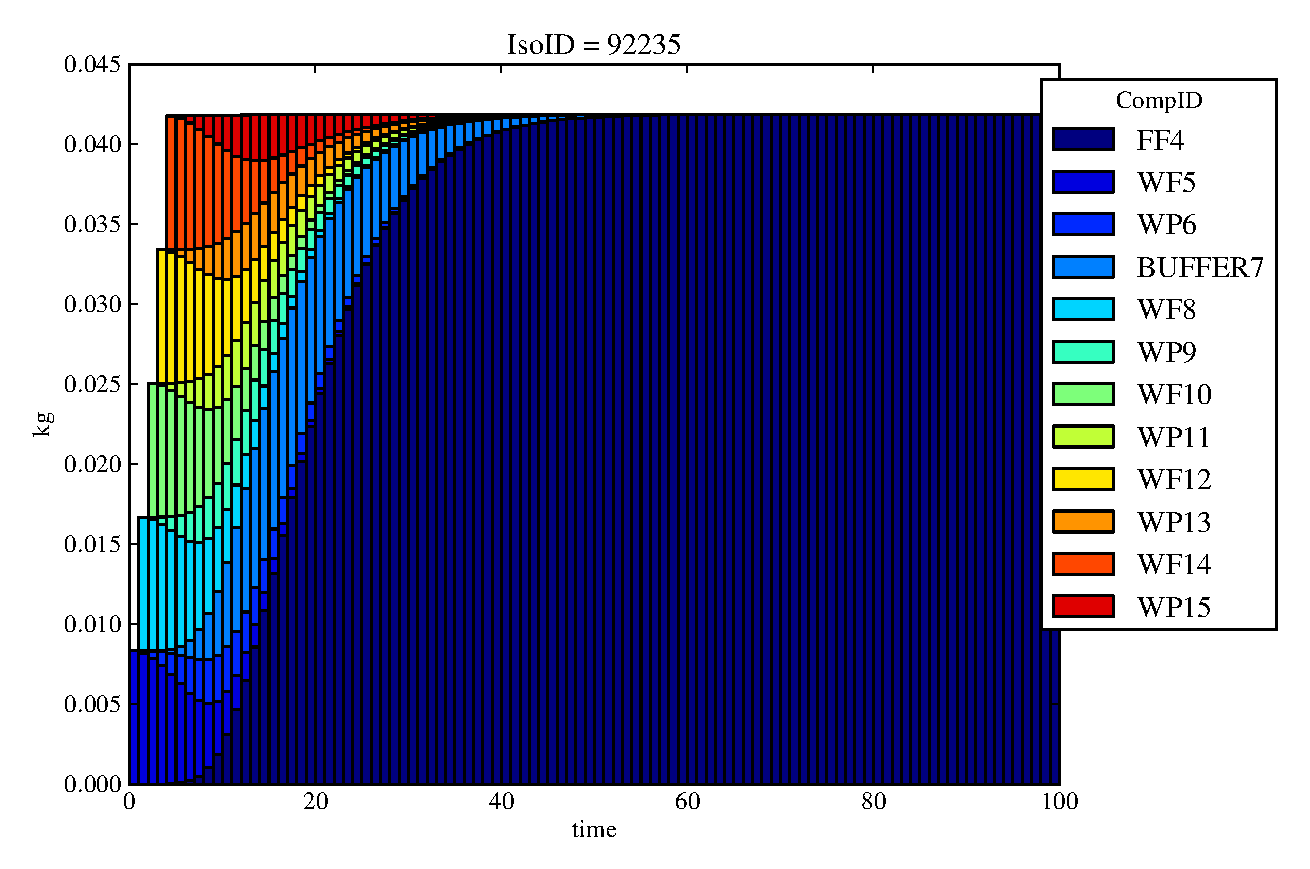
\includegraphics[width=0.6\textwidth]{./results/images/mcIII.eps}
\caption[$^{235}U$ residence. Mixed Cell Coupled Sorption and Solubility Limitation.]{
For the MCIII case in which containment is affected by solubility limitation,
        ($F_{d}=0.1$ for all components except far field), $^{235}U$ travels through waste 
        packages (WPN), their corresponding waste forms (WFN), and the surrounding 
        buffer (BUFFER7) more slowly than in the MCI case
        before permanent residence in the far field component (FF).
}
\label{fig:mcIIIall}
\end{figure}

\begin{figure}[ht]
\centering
  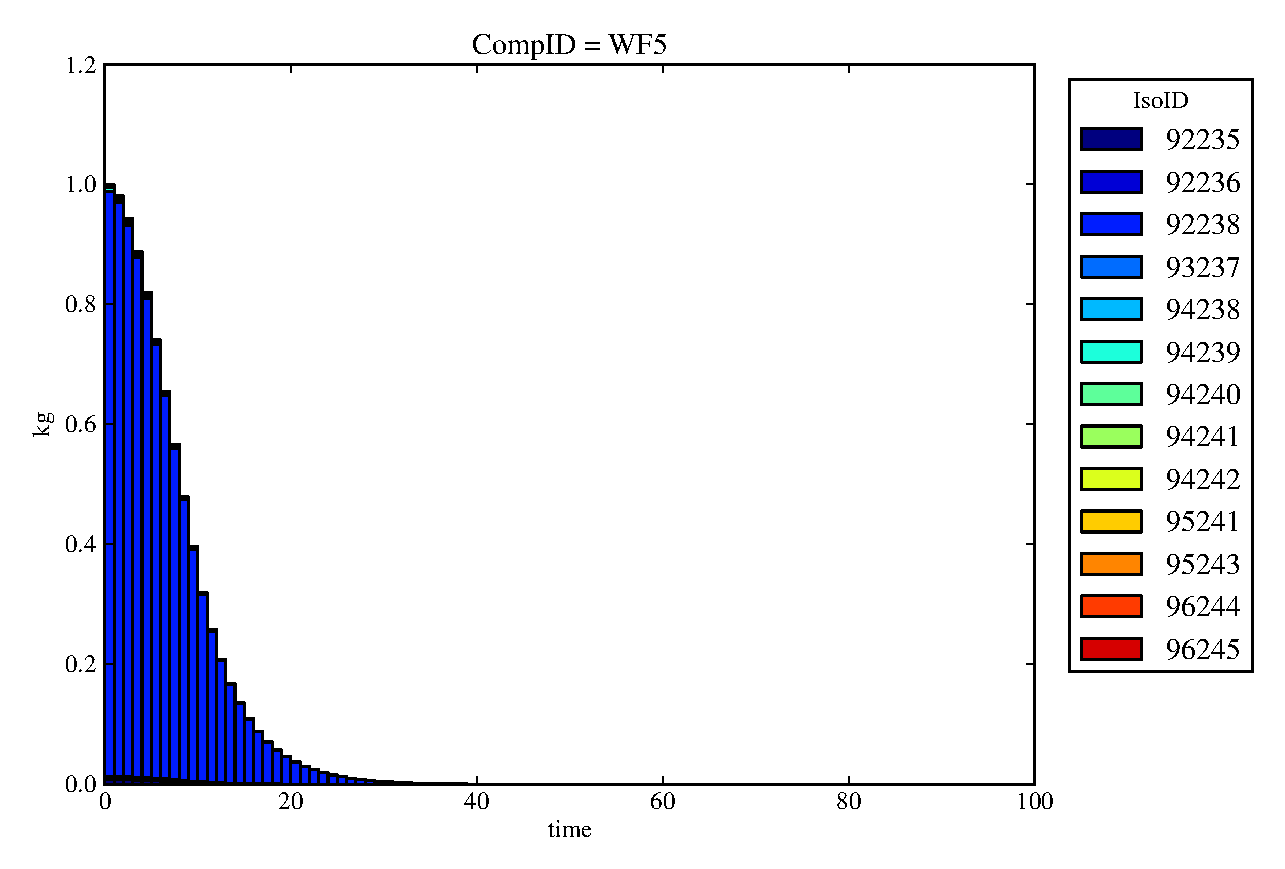
\includegraphics[width=0.6\textwidth]{./results/images/mcIII1.eps}
  \caption[Case MCIII Waste Form Contaminants.]{
          Waste Form 5 (degradation rate $F_d = 0.1[y^{-1}]$, reference solubility limit $S_{ref} = 0.001kg/m^3$) releases material with degradation.
    }
  \label{fig:mcIIIwf5}
\end{figure}


\begin{figure}[ht]
\centering
  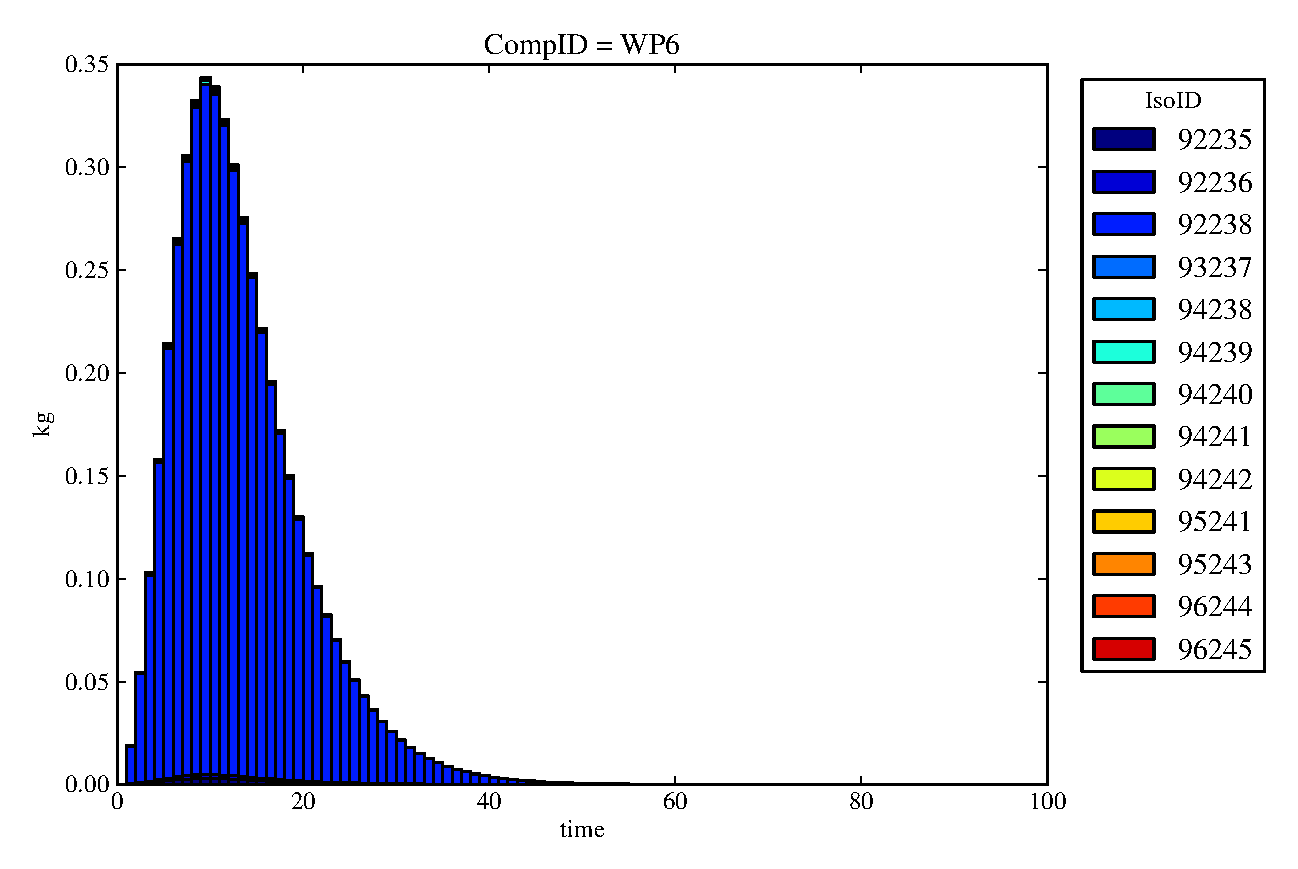
\includegraphics[width=0.6\textwidth]{./results/images/mcIII2.eps}
  \caption[Case MCIII Waste Package Contaminants.]{
          Waste Package 6 (degradation rate $F_d = 0.1[y^{-1}]$, reference solubility limit $S_{ref}=0.001kg/m^3$) receives then releases material.
    }
  \label{fig:mcIIIwp6}
\end{figure}

\begin{figure}[ht]
\centering
  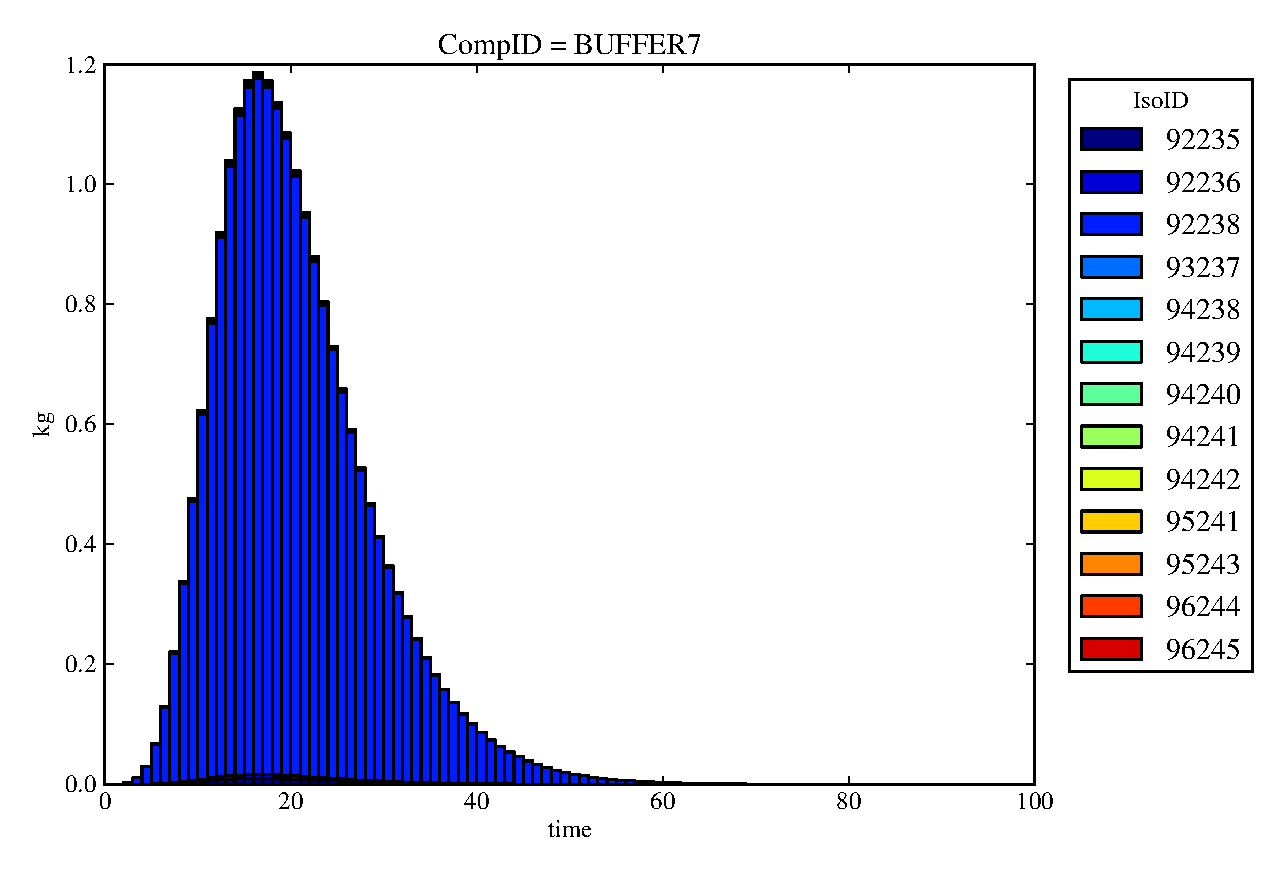
\includegraphics[width=0.6\textwidth]{./results/images/mcIII3.eps}
  \caption[Case MCIII Buffer Contaminants]{
          The Buffer, component 7 (degradation rate $F_d=0.1[y^{-1}]$, reference solubility 
        limit $S_{ref}=0.001kg/m^3$), receives and then releases material.
    }
  \label{fig:mcIIIbuff}
\end{figure}

\begin{figure}[ht]
\centering
  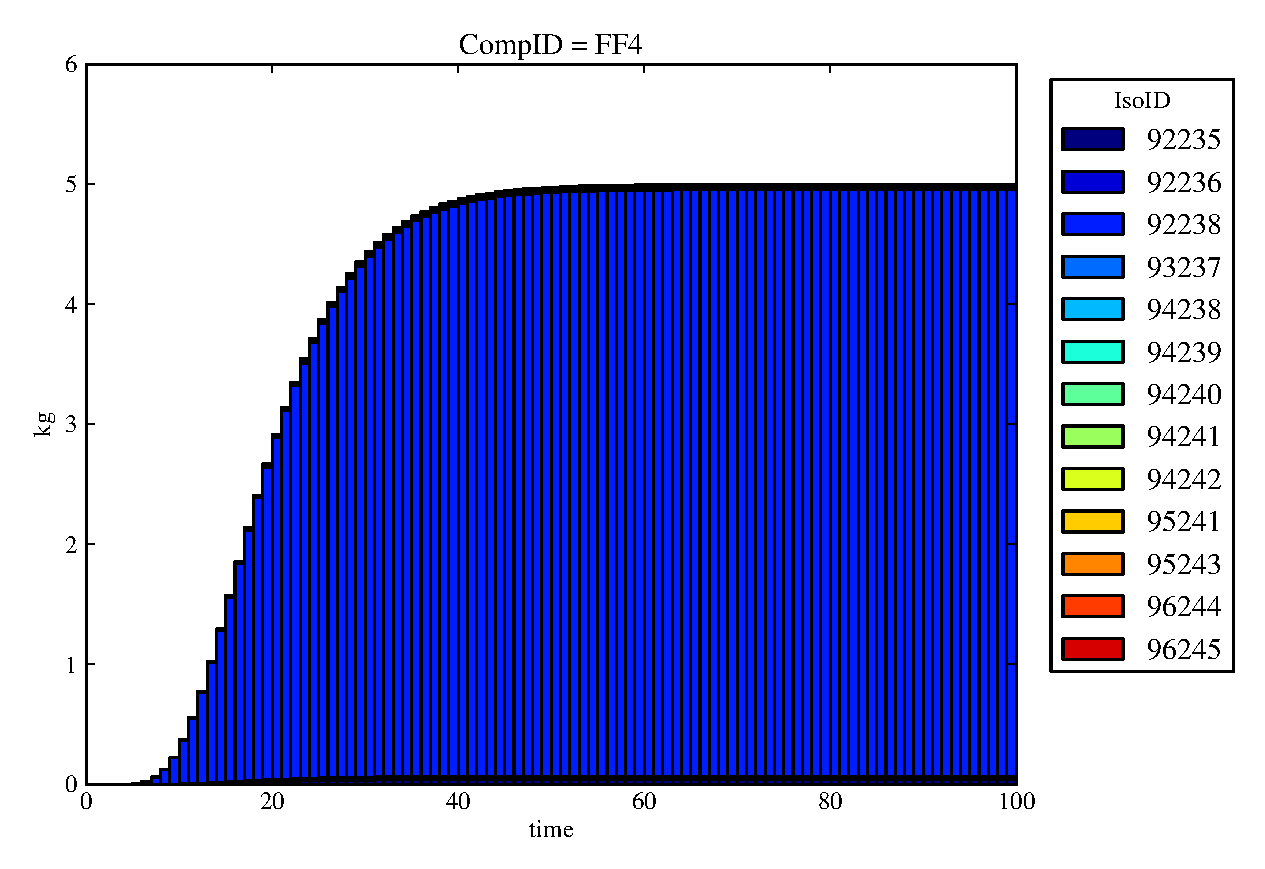
\includegraphics[width=0.6\textwidth]{./results/images/mcIII0.eps}
  \caption[Case MCIII Far Field Contaminants.]{All material is released into
        the Far Field, component 4 (degradation rate $F_d=0.0[y^{-1}]$, reference solubility limit $S_{ref} = 0.001kg/m^3$).}
  \label{fig:mcIII}
\end{figure}



\FloatBarrier

